\subsection{KI, ML, DL - Unterschiede}

Im Zusammenhang mit maschinellem Lernen werden oft die Begrifflichkeiten ''Künstliche Intelligenz'', ''Machine Learning'' und ''Deep Learning'' verwechselt, jedoch handelt es sich bei diesen um eigene Bereiche, die sich in vielen Punkten überschneiden.

\begin{figure}[h b]
    \centering
    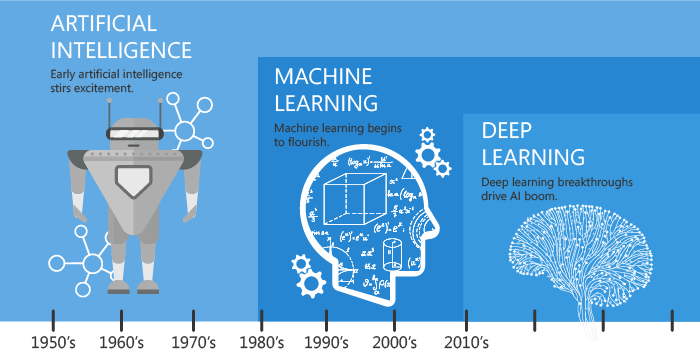
\includegraphics[scale=0.55]{sections/machine-learning/images/ki-ml-dl.png}
    \caption{Evolution von Künstlicher Intelligenz}
    \label{fig:kimldl-comparison}
\end{figure}
%https://miro.medium.com/max/700/0*jng0i9svVVe7L7sj

\subsubsection{KI - Künstliche Intelligenz}

Bereits in den 1950er erschien der Begriff ''Künstliche Intelligenz'', auf englisch ''Artificial Intelligence'', im Bereich Informatik, um Aufgaben zu lösen. Anfänglich noch mit dem Brettspiel "Dame" und einfachen Logikaufgaben. Jedoch kann es sich bei einer KI nur um eine programmierte Regel handeln, da man nur erwartet, dass sich die KI in gewissen Situationen auf eine bestimmte Art und Weise reagiert. Daher beschreibt es Programme, die humane Funktionen, imitieren und gibt nicht an mit welcher Technik das Problem gelöst wird. 

\subsubsection{ML - Machine Learning}

Der Unterschied zur Künstlichen Intelligenz liegt beim Vorgang des Lernens. Genau wie ein menschliches Gehirn muss ein Machine Learning Model mit Daten trainiert werden, mit welchen das Model dann gewisse Klassifizierungen, Clusterbildungen oder Regressionen durchführen kann. Über die Zeit verbessert sich die Präzision, da diese mit Zuwachs der eingespielten Daten wächst.

\subsubsection{DL - Deep Learning}

Sowie beim Machine Learning sind Deep Learning Algorithmen abhängig von antrainierten Daten und kann daher als Synonym oder Untergruppe vom Machine Learning gesehen werden. Jedoch kann ein DL Model wie ein Mensch noch nie davor gesehene spezielle Bilder kategorisieren und ist damit einem ML-Modell in vielen Hinsichten überlegen. 

Ohne Deep Learning würden die meisten modernen Assistenten nicht auf dem Niveau arbeiten wie erwartet, dabei handelt es sich bei Deep Learning um eine junge Technologie, die auf Neuronale Netzwerke basiert.

\paragraph{ML vs DL}

\subparagraph{Feature Extraction}

\begin{figure}[h]
    \centering
    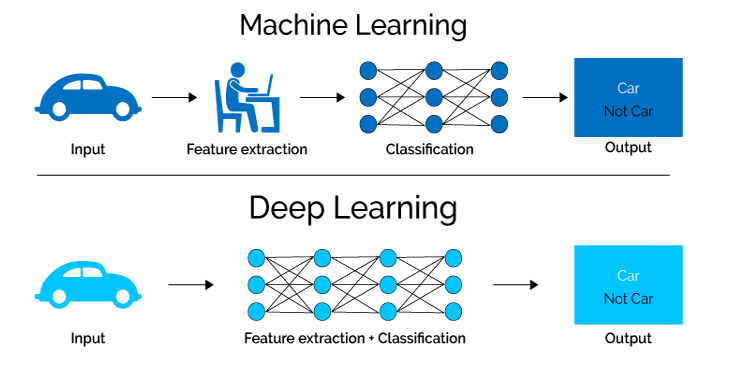
\includegraphics[scale=0.6]{sections/machine-learning/images/MLvsDL.png}
    \caption{Feature Extraction, ML vs DL}
    \label{fig:kimldl-comparison}
\end{figure}

Bevor ein ML-Modell mit der eigentlichen Verarbeitung beginnen kann, müssen die Rohdaten einer sogenannten "Feature Extraction" unterlaufen, welche die gegebenen Daten abstrakt darstellt. Dieser Prozess ist oft sehr kompliziert und beansprucht eine lange Zeit, außerdem ist hier eine Person notwendig, die sich in dem gegebenen Bereich auskennt.

Im Kontrast dazu gibt es Neuronale Netzwerke, welche den Feature Extraction Schritt übernehmen und selbstständig Rohdaten verarbeitet. Über mehrere Schichten werden bestimmte Merkmale hierarchisch definiert und später zum Beispiel zur Kategorisierung genutzt, hierbei erhöht sich die Genauigkeit der Extrahierung schon während des Antrainierens.

\subparagraph{Welches Verfahren ist sinvoller?}

In Bereichen, wo bereits strukturierte Daten vorhanden sind, bietet sind ein ML-Modell an, ein gutes Beispiel dafür ist die Erstellung von Vorhersehung von Ereignissen. Außerdem benötigt man keine große Menge an Daten, um genaue Ergebnise zu bekommen.

Stehen keine bereits vorpreperierte Daten zur Verfügung, wäre ein DL-Modell die bessere Lösung, aber dies auch nur wenn man eine große Menge an Daten hat.